
% !TeX spellcheck = en

\chapter{Flyway vs. Liquibase}

In this section we aim to compare Flyway and Liquibase according to sources \cite{Parsick2018}, \cite{Kaps2016}, \cite{LiquibaseVSFlyway}, \cite{Zylinski2022} and our personal experience gained during this seminar.\\

\section{Comparison}
\marginpar{Commonalities}%
First of all, both tools use a migration-based approach for changes and are open source (Apache v2  \footnote{\url{https://github.com/flyway/flyway/blob/main/LICENSE.txt}} \footnote{\url{https://github.com/liquibase/liquibase/blob/master/LICENSE.txt}}) and in our opinion very easy to use and light-weighted.
Both offer things like repeatable migrations, checksum validation, placeholder replacement and are cluster-safe.
In addition, both tools provide the common interfaces such as CLI, Java API, Maven, Ant, Spring etc.
The list of supported databases is largely the same for both systems, with only minor variations in supported versions or drivers. In general, there are no significant differences in terms of database support between the two systems.


\marginpar{Popularity}%
\textbf{Community}\\
Both have a similarly large community according to the refrences Github stars (Flyway: 6900, Liquibase: 3600) or tags on Stack overflow (Flyway: 2118, Liquibase 3530). 

The search queries on Google also show that both receive a similar number of requests, but Liquibase is slightly ahead. The increase in searches in December 2021 is due to improvements in data collection. 
\begin{figure}[H]
	\centering
	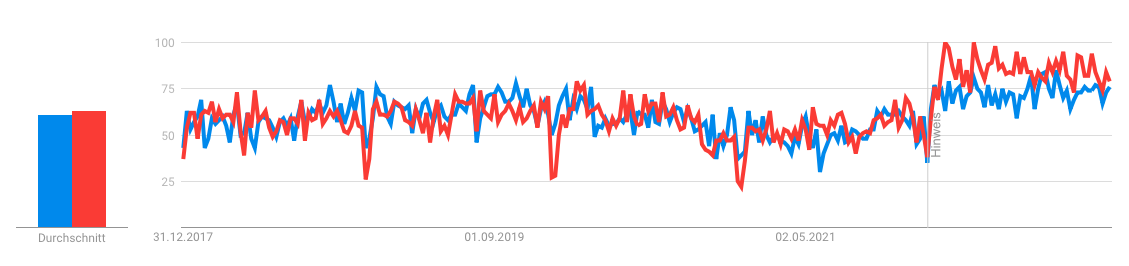
\includegraphics[width=0.9\textwidth]{./chapters/flyway_vs_liquibase/images/flyway_liquibase_search_history}
	\caption[Google Search interest over time - Source: Google Trends]{Google Search interest over time - Source: \url{trends.google.com}}
	% \label{fig:bsp_chapter:example_figure}
\end{figure}


\textbf{Integration into existing projects}\\
In order to be able to integrate existing projects in with flyway, one has to create a manual dump (DDL) of the production database as version 1 script, first clean and empty all other databases and migrate to version 1. Alternatively, you can manually bring the other databases to the state of the production database and set the state as version 1 using the baseline command.\\
On the other hand, in Liquibase it works the following. To tag the state of the production database as version 1, use the \package{generateChangelog} command. To compare the production database with other environments, use the diff command and generate changelogs for any differences. You can mark the generated changelogs as "already run" or exclude them from future runs as needed.\\
LiquiBase integration is highly promising due to the clever combination of its powerful functions. The integration of flyway seems more like a workaround solution.\\

\textbf{Functionalities}\\
In the table x you can see that Liquibase has more functionalities in the ratio 16/9. 

\begin{table}[H]
	\centering
	\begin{tabularx}{10cm}{X c c}
			\rowcolor{black}
		\textcolor{white}{Function}  & 	\textcolor{white}{Flyway} & \textcolor{white}{Liquibase} \\
		\rowcolor{lightgray}
		Migration & +++ & +++ \\ \rowcolor{lightgray}
		& \package{migrate} & \package{update} \\ 
		
		Rollback & - & ++ \\
		& \package{undo} (pro version) & \package{rollback} \\ 	\rowcolor{lightgray}
		
		Clear schema & + & + \\ 	\rowcolor{lightgray}
		& \package{clean} & \package{dropAll} \\
		
		Documentation & + & ++ \\
		& \package{info} & \package{DBDoc} \\ 	\rowcolor{lightgray}
		
		Comparison & - & ++ \\ 	\rowcolor{lightgray}
		&  & \package{Diff} \\
		
		Validation & + & - \\
		& \package{validate} & \\ \rowcolor{lightgray}
		
		Initialization & + & - \\ \rowcolor{lightgray}
		& \package{baseline} & \\
		
		Maintenance & + & + \\
		& \package{repair} & \package{clearChecksums} \\ \rowcolor{lightgray}
		
		Callbacks & + & -\\ \rowcolor{lightgray}
		& & \\
		
		Preconditions & - & + \\
		& & \\ \rowcolor{lightgray}
		
		Context & - & ++ \\ \rowcolor{lightgray}
		& & \\
		
		Refactoring & - & ++ \\
		& & \\
		
	\end{tabularx}
	\caption{Functionalities Flyway vs. Liquibase - Based on \cite{Zylinski2022}}
	\label{tab:functionalities_flyway_liquibase}
\end{table}





\begin{table}[H]
	\centering
		    \begin{tabular}{|l|p{.45\textwidth}|p{.45\textwidth}|}
		    \toprule
			 & Liquibase & Flyway\\ \hline
			 \begin{turn}{-90}Advantages\end{turn} &
			\begin{itemize}
				\item More functionalities such as diff generation (compare two databases), Rollbacks, or monitoring and dashbording possibilities
				\item Apply the same scripts to different database vendors
				\item Integration of existing databases is more promising
				\item Work with NoSQL and relational database types
				\item DDL abstraction DSL (todo: ?)
				\item More flexible when it comes to deployment (selective deployments and rollbacks)
			\end{itemize} & \begin{itemize}
				\item Very easy and intuitive to use
				\item Direct use of SQL files
				\item Multiple schema support (?)
				\item Clean existing schema
				\item Generates SQL for you (?)
			\end{itemize}\\ \hline
		
	 \begin{turn}{-90}Disadvantages\end{turn} &
		\begin{itemize}
			\item Steeper learning curve and more complicated 
			\item No direct support for Java migrations
		\end{itemize} & \begin{itemize}
			\item Important features like Undo or Dry-Run are not included in the free version 
			\item No support for older Java version such as Java 6 \& 7 (enterprise only) (todo: true?)
			\item Versioning system with linear naming convention makes it hard to manage the order of changes
		\end{itemize}\\ \hline
		\end{tabular}
	\caption{Flyway vs Liquibase comparison - Based on \cite{Parsick2018}, \cite{Kaps2016}}
	\label{tab:flyway_liquivase_conparison}
\end{table}


\section{When to use which?}

\marginpar{Question for Selection\\ \cite{Zylinski2022}, \cite{LiquibaseVSFlyway}}%
Even though both provide the basic change management functions perfectly,
there are specific differences in their use. With the following questions the selection can be summed up:

\textit{Does the project use a specific database that only one tool supports?}\\
At the beginning, the framework conditions should be checked whether a certain tool can be used at all. For example, if you also want to integrate NoSQL databases, only Liquibase and not Flyway offers this.

\textit{Do you want to continue using your previous SQL scripts 1:1?}\\
With Flyway, SQL scripts can be integrated directly. Only the name of the script would have to be adapted. When using Liquibase, the changelog files would have to be rewritten again.

\textit{Is it possible to do without rollbacks? (e.g. through clever forward migrations)}\\
Since Flyway does not offer rollbacks in the free version, the choice would fall on Liquibase. However, if you can work around this, there is no disadvantage to using Flyway in this regard.

\textit{Do you need German support?}\\
Since Liquibase is an American company, it provides information in English only. Flyway offers support in several languages and also in German.

\textit{Do you want to have your test data managed as well?}\\
\todo{..}

\textit{Do you want to support diverse DBMS?}\\
Liquibase allows you to use XML, YAML, or JSON to define your database changes, providing an abstraction layer that makes it better suited for use in software products that may be installed in different environments with different underlying database technologies. With Flyway one writes the migrations directly in the SQL language of the used database, therefore with flyway you would have to rewrite the scripts for another database. Probably a lot can be taken over, but there is no guarantee what ends in a manual additional effort.
\vspace{0.5cm}

\textit{Are there many different environments with different database schema requirements?}\\
If this is a requirement, Liquibase is the tool of choice because one can selectively deploy changes as needed to different environments. 
Liquibase offers support for updating and managing the same schema across multiple database vendors \& platforms using the same changelog file.
In addition there is support to easily add new changes and reorder them without running into filename conflicts

\textit{How large is the development team?}\\
\todo{..}


\newpage